\documentclass{article}
\usepackage{import}
\usepackage{amsmath}
\usepackage{tabularray}
\usepackage{float}


\import{lib/latex/}{wgmlgz}
\patchcmd{\thebibliography}{\section*}{\section}{}{}

\begin{document}
\itmo[
      variant=13,
      labn=1,
      discipline=Вычислительная математика,
      group=P3212,
      student=Соколов Анатолий Владимирович,
      teacher=Наумова Надежда Александровна 
]
\lstset{language=rust}
\newgeometry{
  a4paper,
  top=20mm,
  right=10mm,
  bottom=20mm,
  left=30mm
}
\tableofcontents

\section{Задание}
% \begin{enumerate}
      В программе реализуемый численный метод решения системы линейных алгебраических уравнений (СЛАУ) должен быть реализован в виде отдельного класса /метода/функции, в который исходные/выходные данные передаются в качестве параметров.
      \\
      Задавать размерность матрицы ($n<20$) из файла или с клавиатуры ‒ по выбору конечного пользователя.
      \\      
      Должна быть реализована возможность ввода коэффициентов матрицы, как с клавиатуры, так и из файла (по выбору конечного пользователя).
      \\
      Сформировать не менее 3 файлов (тестов) с различным набором данных.
      \\
      Программа должна быть протестирована на различных наборах данных, в том числе и некорректных.

\subsection{Вариант}

\textbf{Для итерационных методов должно быть реализовано:}

\begin{center}
      % \includegraphics[width=175pt]{opd/4/4.png}
      \begin{itemize}
      \item Точность задается с клавиатуры/файла
      \item Проверка диагонального преобладания (в случае, если диагональное преобладание в исходной матрице отсутствует, сделать перестановку строк/столбцов до тех пор, пока преобладание не будет достигнуто). В случае невозможности достижения диагонального преобладания - выводить соответствующее сообщение.
      \item Вывод вектора неизвестных: $x1$, $x2$, $\dots$ , $x_n$
      \item Вывод количества итераций, за которое было найдено решение.
      \item Вывод вектора погрешностей: $|x_i^K-x_i^{k-1}|$
      \end{itemize}
\end{center}

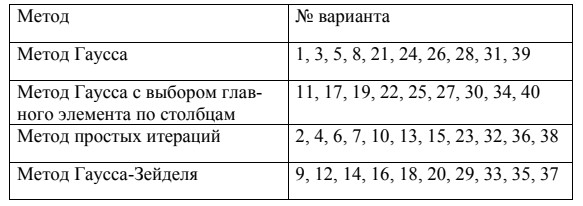
\includegraphics{task.jpg}

\subsection{Цель работы}
      Рассчитать систему линейных алгебраических уравнений СЛАУ и изучить МПИ.

\subsection{Описание метода, расчетные формулы}
      \textbf{Описание метода}
      \\
      Итерационные методы это методы последовательных приближений.
      \\
      Задается некоторое начальное приближение. Далее с помощью определенного алгоритма проводится один цикл вычислений - итерация. В результате итерации находят новое приближение. Итерации проводятся до получения решения с требуемой точностью.
      \\
      Метод простых итераций — это численный метод решения уравнений, включая алгебраические и дифференциальные уравнения. Основная идея метода состоит в том, чтобы преобразовать исходное уравнение таким образом, чтобы решение могло быть представлено как предел последовательности, получаемой итеративным способом.
      \\
      Для алгебраических уравнений метод простых итераций можно описать следующим образом:
      \\
      1. Преобразование уравнения: Исходное уравнение \(f(x) = 0\) преобразуется в эквивалентное уравнение вида \(x = \phi(x)\), где функция \(\phi(x)\) должна быть выбрана таким образом, чтобы последовательность, порождаемая этой функцией, сходилась к корню исходного уравнения.
      \\
      2. Выбор начального приближения: Выбирается начальное приближение к корню уравнения, обозначаемое как \(x_0\).
      \\
      3. Итерационный процесс: На каждом шаге вычисляется следующее приближение к корню по формуле \(x_{n+1} = \phi(x_n)\), где \(n\) — номер текущей итерации. Этот процесс повторяется до тех пор, пока разность между последовательными приближениями не станет меньше заданной точности \(\varepsilon\), т.е. \(|x_{n+1} - x_n| < \varepsilon\).
      \\
      4. Критерий остановки: Итерационный процесс продолжается до тех пор, пока не будет достигнута заданная точность или не будет выполнено максимально допустимое количество итераций.
      \\
      \textbf{Расчетные формулы}

      $$x_i^{k+1}=\frac{b_i}{a_{ii}}-\sum_{j=1, j \neq i}^n \frac{a_{ij}}{a_{ii}}x^k_j, i = 1,2,\dots,n$$
      $$c_{ij}=
      \begin{cases}
            0, i=j\\
            -\frac{a_{ij}}{a_{ii}}
      \end{cases}$$
      $$d_i=\frac{b_i}{a_{ii}}, i=1,2,\dots,n$$
      $$x^{k+1}=Cx^k+d$$

\subsection{Реализация численного метода}
\begin{lstlisting}
fn shuffle(&mut self) -> (bool, Vec<Vec<f64>>) {
      let mut biggest = vec![-1; self.n];
      let mut biggest_set = HashSet::new();
      let mut found_strict = false;

      for i in 0..self.n {
            let sum: f64 = self.a[i].iter().sum();
            for j in 0..self.n {
                  if 2.0 * self.a[i][j] >= sum {
                  if 2.0 * self.a[i][j] > sum {
                        found_strict = true;
                  }
                  biggest[i] = j as isize;
                  biggest_set.insert(j);
                  break;
                  }
            }
            if biggest[i] == -1 {
                  return (false, vec![vec![0.0]]);
            }
      }

      if !found_strict || biggest.len() != biggest_set.len() {
            return (false, vec![vec![0.0]]);
      }

      let mut shuffled_a = vec![vec![]; self.n];
      let mut shuffled_b = vec![0.0; self.n];

      for i in 0..self.n {
            let index = biggest[i] as usize;
            shuffled_a[index] = self.a[i].clone();
            shuffled_b[index] = self.b[i];
      }

      self.a = shuffled_a.clone();
      self.b = shuffled_b;

      (true, shuffled_a)
      }

fn find_c_and_d(coefficients: Vec<Vec<f64>>) -> Vec<Vec<f64>> {
      let n = coefficients.len(); // The number of rows, assuming a square matrix for coefficients
      let mut c = vec![vec![0.0; n]; n]; // Initialize C matrix with zeros

      for i in 0..n {
            // Diagonal element of the current row
            let diag_elem = coefficients[i][i];

            for j in 0..n {
                  // Check if the current element is not on the diagonal
                  if i != j {
                  // C matrix is -1 times the original coefficient matrix divided by the diagonal element
                  c[i][j] = -coefficients[i][j] / diag_elem;
                  }
            }
            // The diagonal elements of C are set to zero
            c[i][i] = 0.0;
      }

      c
      }

fn iterate(&mut self) {
      let mut new_sol = vec![0.0; self.n];
      for i in 0..self.n {
            new_sol[i] = self.b[i] / self.a[i][i] - self.sum_sol_row(i);
            self.sol_acc[i] = (new_sol[i] - self.sol[i]).abs();
      }
      self.sol = new_sol;
      self.sol_iter += 1;
      }

      pub fn solve(&mut self) -> Json<serde_json::Value> {
      let mut err = String::new();

      if !self.shuffle().0 {
            err = String::from("Невозможно привести к диагональному преобладанию.")
      }

      self.shuffled_matrix = self.shuffle().1;

      while self.sol_acc.iter().max_by(|a, b| a.total_cmp(b)).unwrap() > &self.acc
            && self.sol_iter < self.max_iter
      {
            self.iterate();
      }

      if !self.shuffled_matrix.is_empty() {
            self.c = Matrix::find_c_and_d(self.shuffle().1);
            return Json(json!({
                  "sol": self.sol,
                  "acc": self.sol_acc,
                  "iter": self.sol_iter,
                  "c": self.c,
                  "mtrx": self.shuffled_matrix,
                  "err": err,
            }));
      }

      Json(json!({
            "sol": self.sol,
            "acc": self.sol_acc,
            "iter": self.sol_iter,
            "mtrx": self.shuffled_matrix,
            "err": err,
      }))
      }
\end{lstlisting}

\subsection{Блок-схема реализованного алгоритма}
      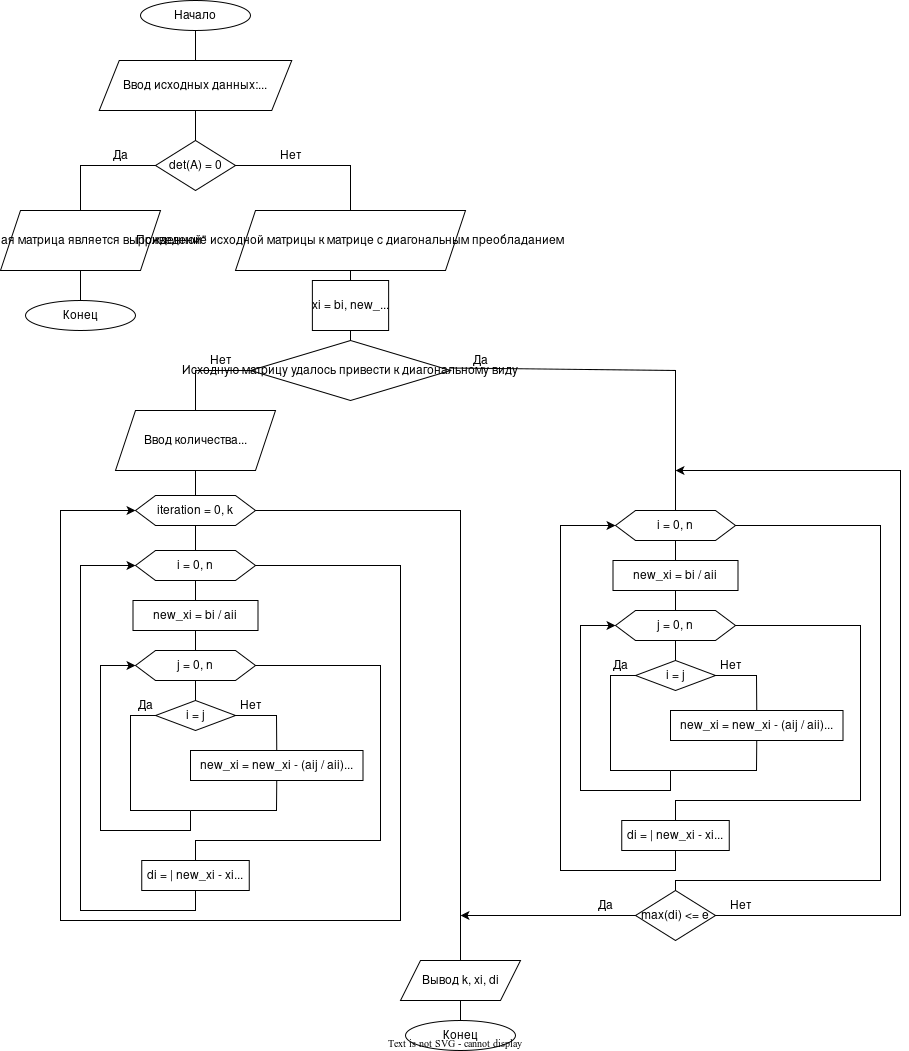
\includegraphics[scale=0.5]{AlgoSheme.png}
\subsection{Ссылка на GitHub c основной реализацией}
      \href{https://github.com/isofinly/compmath}{Github}

\subsection{Примеры и результаты работы программы}
      \begin{center}
            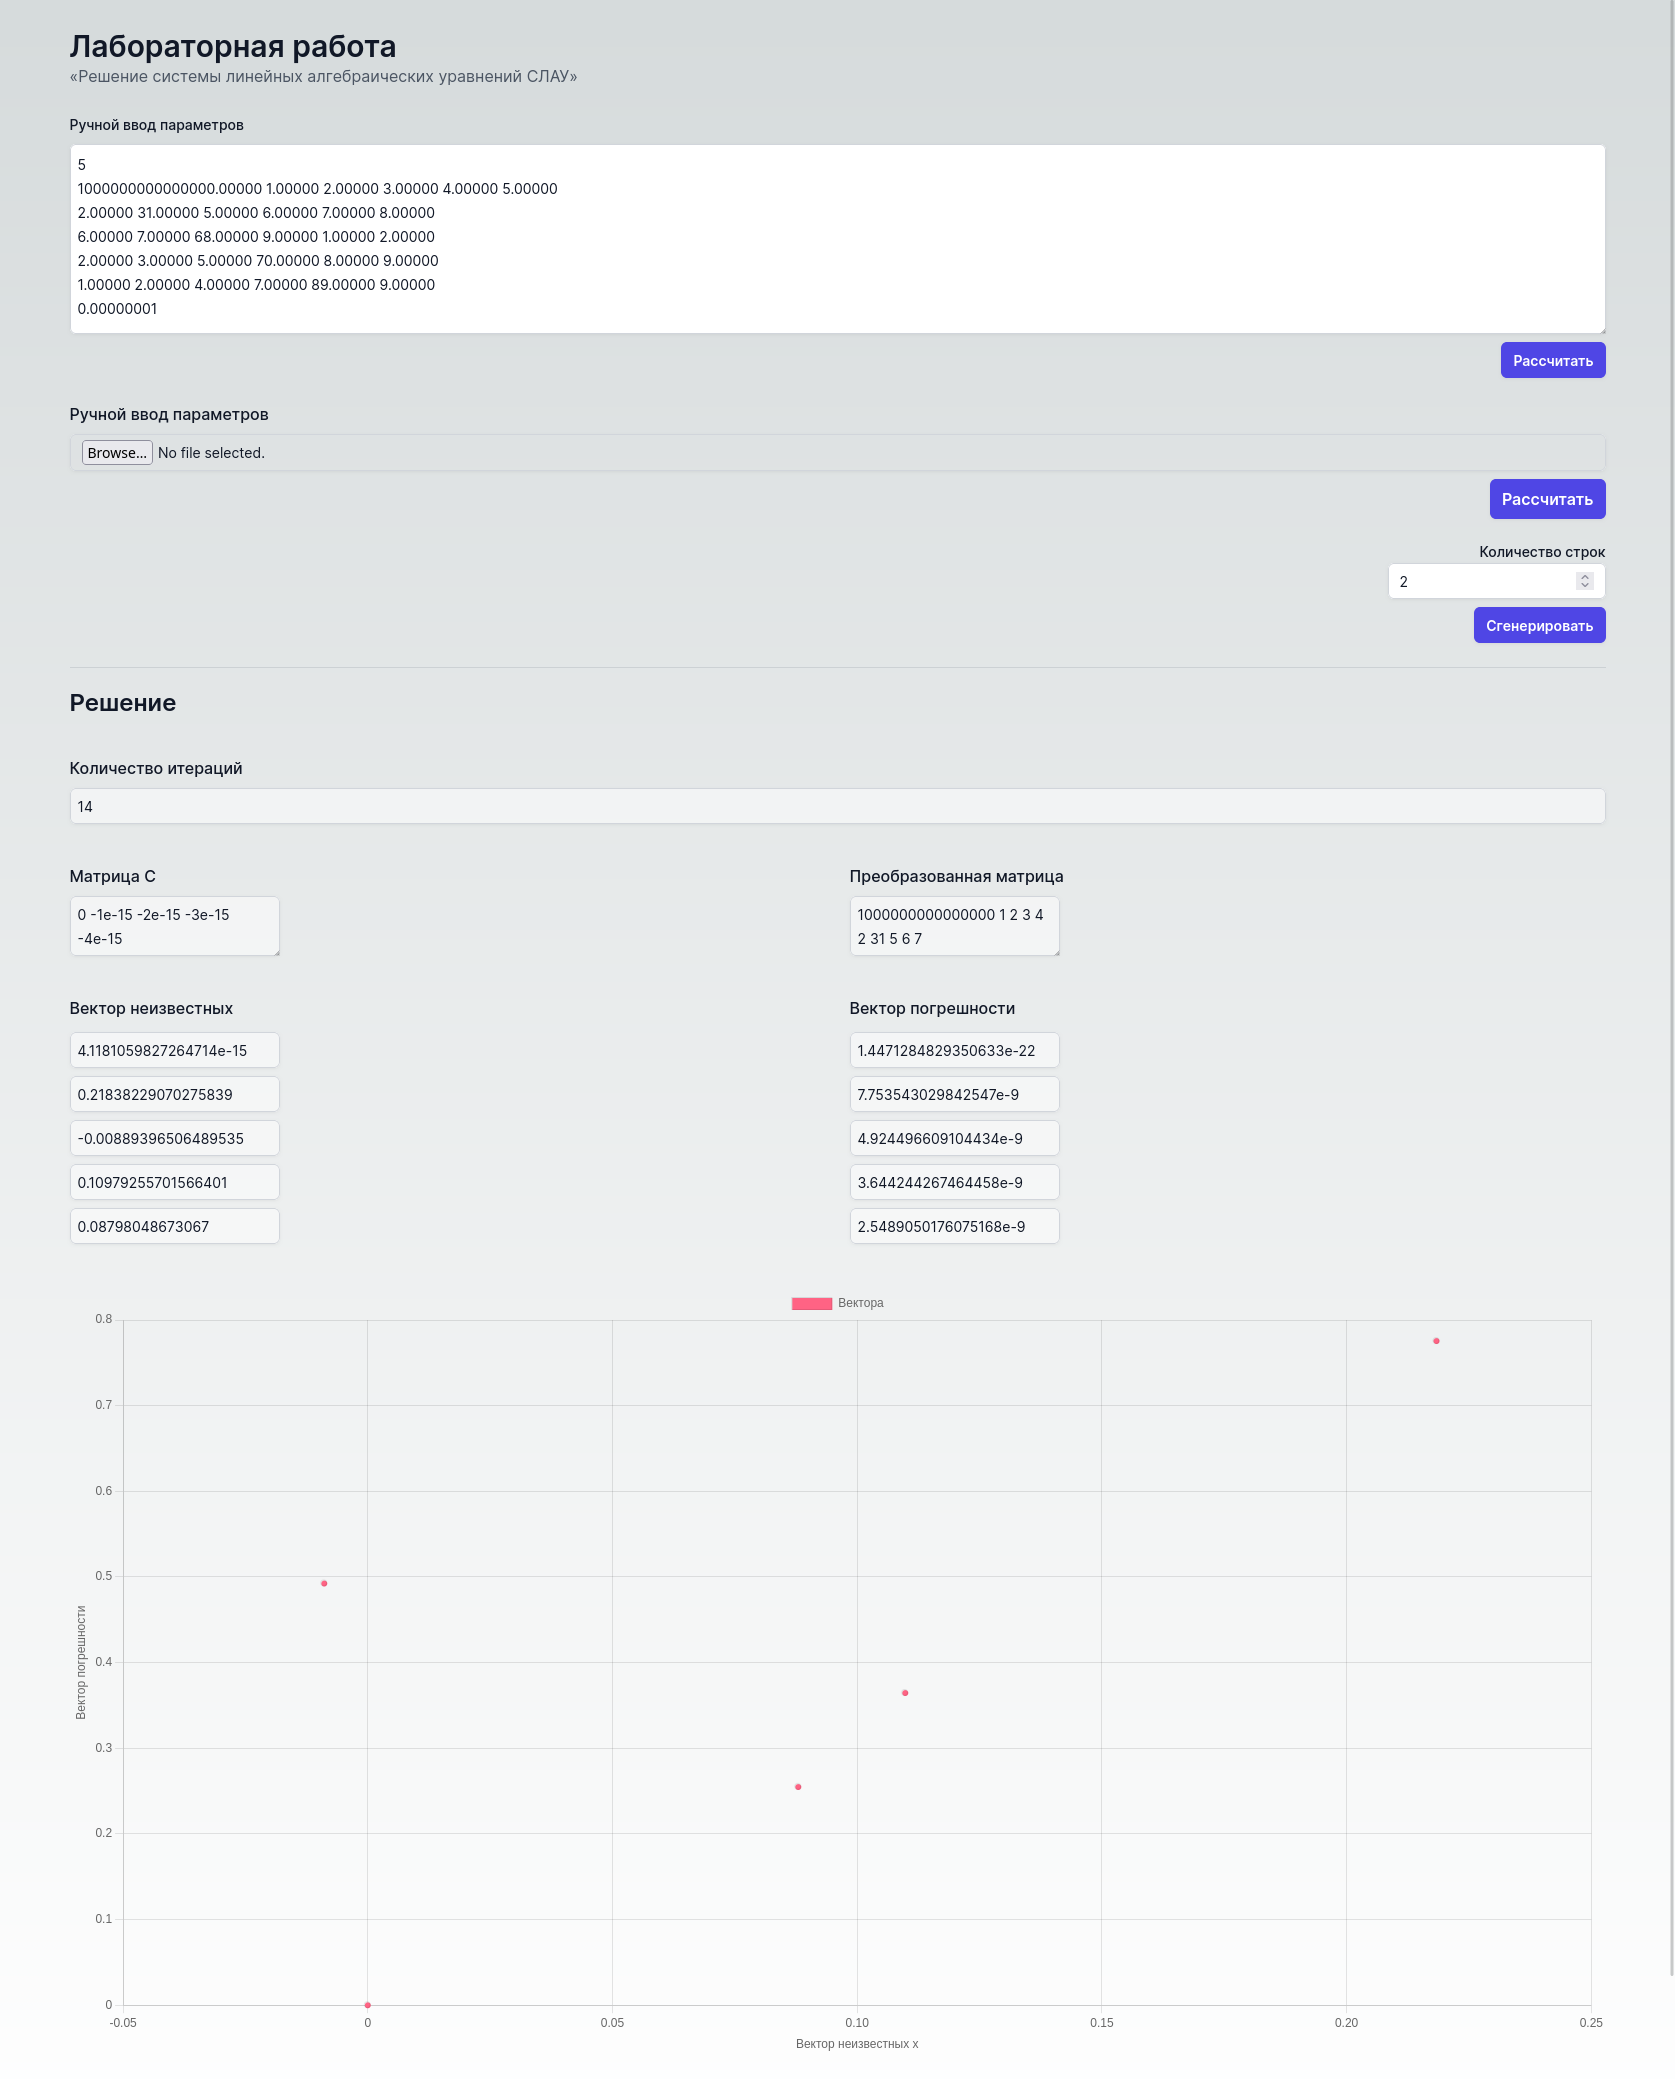
\includegraphics[scale=0.25]{solution1.png}

            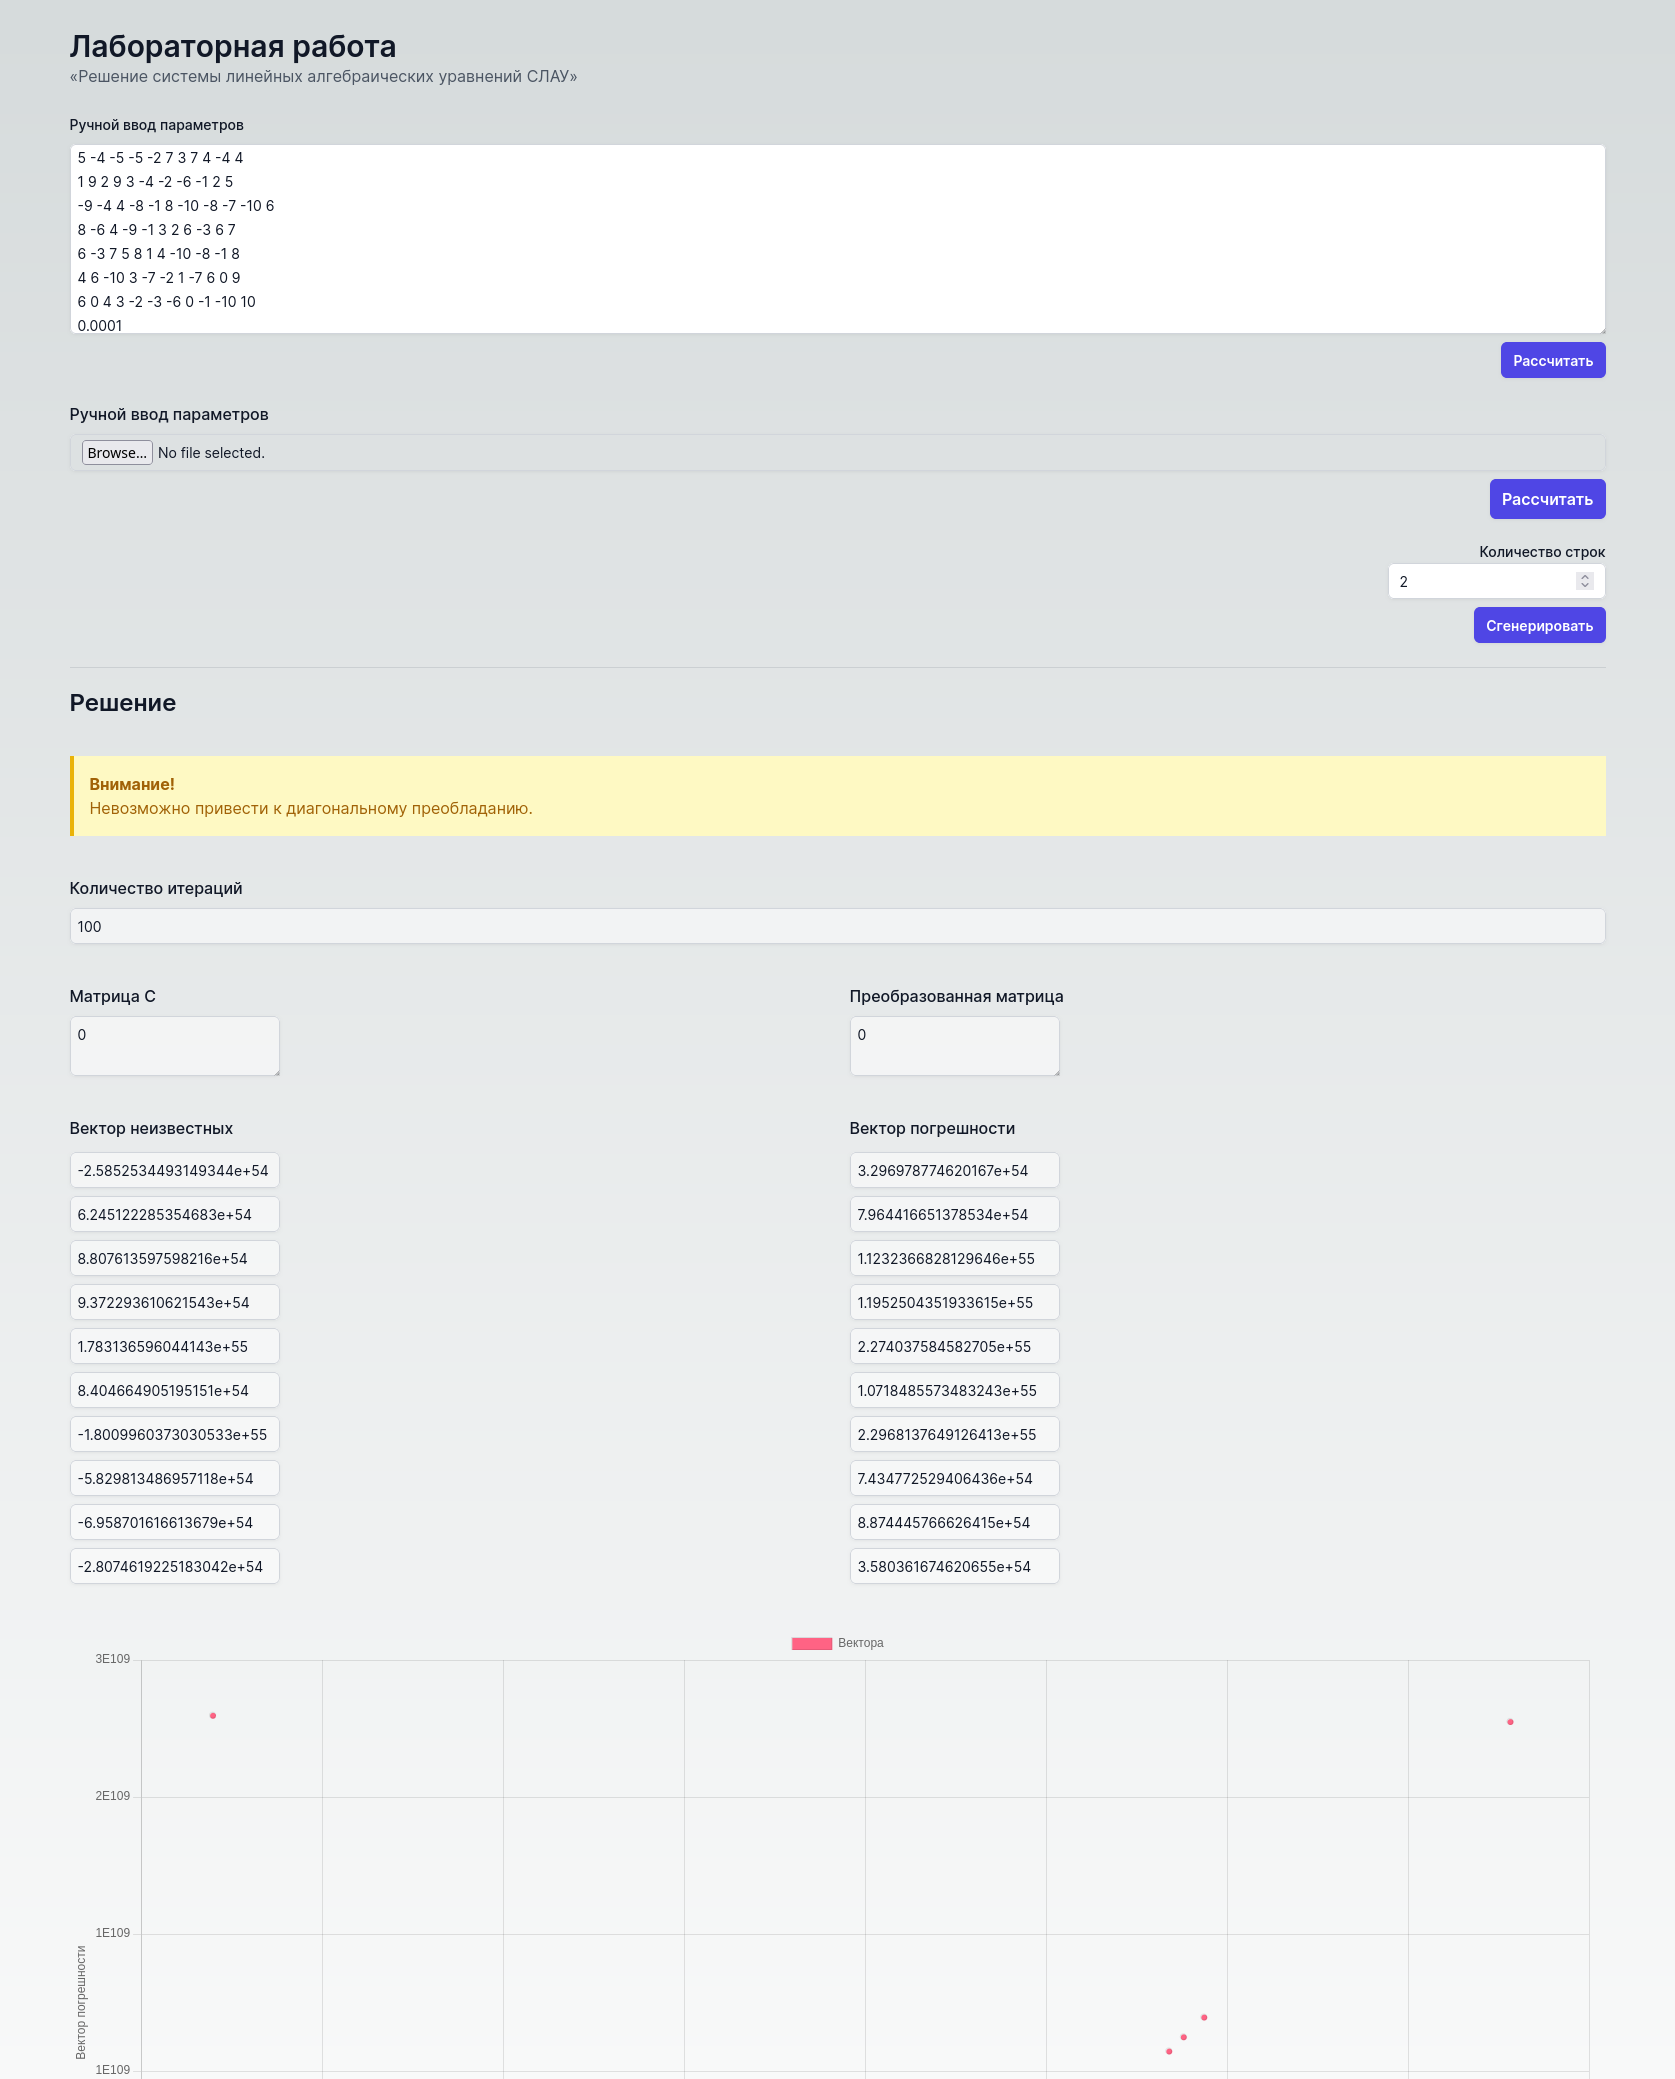
\includegraphics[scale=0.25]{solution2.png}
      \end{center}
      

\section{Заключение}
Я познакомился с новым для меня и крайне необыкновенным вычислением СЛАУ на языке rust.


\begin{thebibliography}{9}
    \bibitem{Методичка}Слайды с лекций (2023). // Кафедра информатики и вычислительной техники -- Малышева Татьяна Алексеевна, к.т.н., доцент.
\end{thebibliography} 

\end{document}
